\hypertarget{section-concepts}{%
\section{Cross-cutting Concepts}\label{section-concepts}}

\textbf{Content}

This section describes overall, principal regulations and solution ideas
that are relevant in multiple parts (= cross-cutting) of your system.
Such concepts are often related to multiple building blocks. They can
include many different topics, such as

\begin{itemize}
\item
  models, especially domain models
\item
  architecture or design patterns
\item
  rules for using specific technology
\item
  principal, often technical decisions of an overarching (=
  cross-cutting) nature
\item
  implementation rules
\end{itemize}

\textbf{Motivation}

Concepts form the basis for \emph{conceptual integrity} (consistency,
homogeneity) of the architecture. Thus, they are an important
contribution to achieve inner qualities of your system.

Some of these concepts cannot be assigned to individual building blocks,
e.g. security or safety.

\textbf{Form}

The form can be varied:

\begin{itemize}
\item
  concept papers with any kind of structure
\item
  cross-cutting model excerpts or scenarios using notations of the
  architecture views
\item
  sample implementations, especially for technical concepts
\item
  reference to typical usage of standard frameworks (e.g. using
  Hibernate for object/relational mapping)
\end{itemize}

\textbf{Structure}

A potential (but not mandatory) structure for this section could be:

\begin{itemize}
\item
  Domain concepts
\item
  User Experience concepts (UX)
\item
  Safety and security concepts
\item
  Architecture and design patterns
\item
  "Under-the-hood"
\item
  development concepts
\item
  operational concepts
\end{itemize}

Note: it might be difficult to assign individual concepts to one
specific topic on this list.

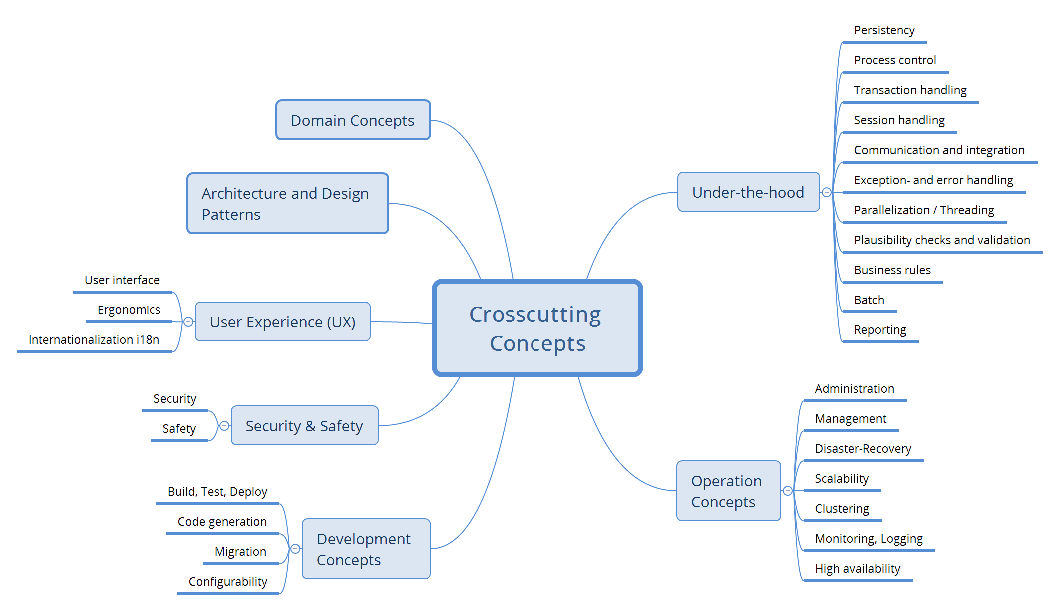
\includegraphics{../images/08-Crosscutting-Concepts-Structure-EN.png}

See \href{https://docs.arc42.org/section-8/}{Concepts} in the arc42
documentation.

\hypertarget{__emphasis_concept_1_emphasis}{%
\subsection{\texorpdfstring{\emph{\textless Concept
1\textgreater{}}}{\textless Concept 1\textgreater{}}}\label{__emphasis_concept_1_emphasis}}

\emph{\textless explanation\textgreater{}}

\hypertarget{__emphasis_concept_2_emphasis}{%
\subsection{\texorpdfstring{\emph{\textless Concept
2\textgreater{}}}{\textless Concept 2\textgreater{}}}\label{__emphasis_concept_2_emphasis}}

\emph{\textless explanation\textgreater{}}

\ldots{}

\hypertarget{__emphasis_concept_n_emphasis}{%
\subsection{\texorpdfstring{\emph{\textless Concept
n\textgreater{}}}{\textless Concept n\textgreater{}}}\label{__emphasis_concept_n_emphasis}}

\emph{\textless explanation\textgreater{}}
